\documentclass{article}
\usepackage{graphicx, xcolor, amsmath, amssymb, amsthm} % Required for inserting images
\usepackage{tikz}
\usepackage{hyperref}
\usetikzlibrary{positioning, arrows.meta, decorations.markings}

% distance to H-freeness
\DeclareMathOperator{\dist}{dist}

% theorem-like environments
\theoremstyle{plain}
\newtheorem{theorem}{Theorem}
\newtheorem{conjecture}[theorem]{Conjecture}
\newtheorem{lemma}[theorem]{Lemma}
\newtheorem{proposition}[theorem]{Proposition}
\newtheorem{corollary}[theorem]{Corollary}
\newtheorem{remark}[theorem]{Remark}

\theoremstyle{definition}
\newtheorem{definition}[theorem]{Definition}
\newtheorem{example}{Example}

\title{Polynomial removal for binary matrices\\
\Large Problem \#96 at the Caltech $\times$ SAIR Mathathon}
\author{Team Name: costco\\
\,\\
Papangkorn Apinyanon, MIT\\
Saksham Sethi, Caltech, and\\
Henning Arn\'or Skeggi \'Ulfarsson, Reykjavik University}
\date{November 15, 2026}

\begin{document}

\maketitle

Team formation TODO

Problem selection TODO

Use of LLMs during our work. Most of the work was carried out in Opus 5.5.
This involved literature search, summarizing and giving examples from existing work, looking for extensions, both in terms of new counterexamples as well as
matrices that have polynomial removal. We briefly used Fable 5.2 for searching for smaller counterexamples. Opus 5.5 and GPT-6.1 Sol was used to orchistrate Lean formalization, in the sense that those agents set up the proofs and prompts for agents running in the Open Math environment. Kimi 3.1 Pro on the Ultramath setting carried out the Lean formalization. Opus 5.5 was also used to formalize a subset of our result in Agda, but we do not include that work here.

In the writing of this report and the accompanying slides we used Opus 5.5 with some help from DeepSeek V4.1 Flash and Kimi 3.1 Pro in the Open Math environment.

All work that was turned in was created at the event. Prior to the event we
read the literature, with help from LLMs

%Running list of models used
%\begin{itemize}
%    \item Literature search, summarizing existing work, hunt for extensions, smaller counterexamples, proofs (matrices that have polynomial removal)
%    \begin{itemize}
%        \item Opus 5.5 (Max)
%        \item Fable 5.2 (Medium)
%    \end{itemize}
%   \item Formalization
%    \begin{itemize}
%        \item GPT-6.1 Sol (Extra High) and Opus 5.5 (Max): Planning which models to use in Open OS to formalize the existence of infinite families of counterexamples, and how to prompt
%        \item Carrying out the Lean formalization: Open Math Kimi 3.1 Pro (Ultramath, subagent type selected by model) for Lean formalization
%        \item Agda formalization of smaller instances: Opus 5.5 (Max)
%    \end{itemize}
%    \item Proof-reading text, help with slides, writing examples
%    \begin{itemize}
%        \item Opus 5.5 (Max)
%        \item Open Math DeepSeek V4.1 Flash and Kimi 3.1 Pro
%    \end{itemize}
%\end{itemize}

\section*{Introduction and Results}
Let $H$ be a $k \times k$ binary matrix. An (\emph{ordered}) \emph{copy} of $H$ in a larger $n \times n$ binary matrix $A$ is a choice of rows $1 \le r_1 < \dots < r_k \le n$ and columns $1 \le c_1 < \dots < c_k \le n$ such that $A(r_i, c_j) = H(i, j)$ for all $i, j$. Notice that this requires both the $0$s and the $1$s of $H$ to be in the correct positions. When such a copy exists we say that $A$ \emph{contains} $H$ (\emph{as an ordered copy}); otherwise $A$ is \emph{$H$-free}.                                                                                                                                                       \begin{example}\label{ex:copies}                                                            Let                                                                                         \[
    H = \begin{pmatrix} 1 & 0 \\1 & 1 \end{pmatrix}                                        \qquad\text{and}\qquad
    A = \begin{pmatrix}
    \boxed{1} & 0 & \boxed{0} \\
    \boxed{1} & 1 & \boxed{1} \\
    1 & 0 & 1
    \end{pmatrix}.
\]
  The boxed entries, in rows $1, 2$ and columns $1, 3$, form a copy of $H$. There are two more copies: rows $1, 2$ with columns $1, 2$, and rows $1, 3$ with columns $1, 3$. There
  are no others.
  \end{example}

  Let $N_H(A)$ be the number of ordered copies of $H$ in $A$, and let $D_H(A)$ be the minimum
  number of entries of $A$ that must be changed so that the resulting matrix is $H$-free. Also let
  $\dist_H(A) = D_H(A)/n^2$. For $\epsilon \le \dist_H(A)$ we say that $A$ is
  \emph{$\epsilon$-far} from being $H$-free, because then at least $\epsilon n^2$ entries need to be
  changed to remove all copies of $H$.

  \begin{example}\label{ex:distance}
  In Example~\ref{ex:copies}, $N_H(A) = 3$. All three copies use the entry $A(1,1)$, highlighted
  below, and changing it to $0$ gives the matrix $A'$:
  \[
  A = \begin{pmatrix}
    \colorbox{yellow!50}{$1$} & 0 & 0 \\
    1 & 1 & 1 \\
    1 & 0 & 1
  \end{pmatrix},
  \qquad
  A' = \begin{pmatrix}
    \colorbox{yellow!50}{$0$} & 0 & 0 \\
    1 & 1 & 1 \\
    1 & 0 & 1
  \end{pmatrix}.
  \]
  The matrix $A'$ is $H$-free. Since $A$ contains $H$, at least one
  change is needed, so $D_H(A) = 1$ and $\dist_H(A) = 1/9$; that is, $A$ is $\epsilon$-far from
  being $H$-free for every $\epsilon \le 1/9$.

  Note that a change can create new
  copies. For instance, changing $A(1,2)$ from $0$ to $1$ destroys one copy
  of Example~\ref{ex:copies}, but rows $1, 2$ with columns $2, 3$ become a new copy, and the other two copies survive, so the result still has three copies.
  \end{example}

 The polynomial ordered binary matrix-removal conjecture was:
 
\begin{conjecture}\label{conj:poly-removal}
For every $k \times k$ binary matrix $H$, there are constant $c, C > 0$, depending only on $H$, such that for every $n$, every $n\times n$ binary matrix $A$ and every $\epsilon \in (0,1]$: if $\dist_H(A) \ge \epsilon$, then $N_H(A) \ge c\epsilon^C n^{2k}$. In other words, if at least $\epsilon n^2$ entries of $A$ need to be changed to remove all copies of $H$, then
$A$ contains at least $c\epsilon^Cn^{2k}$ copies of $H$.
\end{conjecture}

This question was first raised by Alon, Fischer, and Newman in 2007~\cite{AFN}, and Alon and Ben-Eliezer posed it for finite families of patterns in 2020~\cite{ABE}. A weaker removal lemma does hold for this problem, but $\delta^{-1}$ grows like a wowzer-type function of $\epsilon^{-1}$, instead of polynomial Alon, Ben-Eliezer and Fischer 2017~\cite{ABF17}. In Gishboliner and Shapira's survey, they mentioned polynomial removal as a key open problem, and the OpenAI preprint shows it fails for a specific $66 \times 66$ matrix $H$. Later, Wang reduced it to a $4 \times 4$ counterexample \cite{wang}, and thereafter Shea reduced it to a $3 \times 3$ one \cite{shea}. \\

In this paper, we give a conceptual, human-readable exposition of the key theorem from Alon and Ben-Eliezer, and how OpenAI's counterexample works in the context of that framework. Additionally, our novel contributions are two structural theorems about which patterns satisfy the conjecture:
\begin{itemize}
    \item \textit{Duplication}: Theorem 3 shows that repeating a row or column consecutively does not change whether the matrix satisfies the conjecture. 
    \item \textit{Direct Sum}: Theorem 2 shows that if $H$ is a counterexample, doing direct sum with any matrix $Z$ under certain conditions will lead to $H'$, which is another counterexample.
\end{itemize}
We can achieve some results with these reduction-type theorems. Combined with the counterexamples by OpenAI, Shea, Wang, and we give the first infinite family of counterexamples. Additionally, combined with Lupini's result \cite{Lupini}, we also get an infinite family of patterns that satisfy the conjecture. 




\section*{The approach of Alon and Ben-Eliezer, and how $A_h$ escapes it}
  Call copies of $H$ \emph{pairwise disjoint} if no two of them share an entry.
  Alon and Ben-Eliezer proved that if an $n \times n$ matrix $A$ contains
  $\epsilon n^2$ pairwise disjoint copies of $H$, then $N_H(A) \ge \delta n^{2k}$
  with $1/\delta$ polynomial in $1/\epsilon$ \cite[Theorem~1.2]{ABE}. So the
  conjecture would follow if every matrix that is $\epsilon$-far from being
  $H$-free contained $\tau n^2$ pairwise disjoint copies of $H$, with $1/\tau$
  polynomial in $1/\epsilon$. For OpenAI's $66 \times 66$ pattern $H$, the host
  matrices $A_h$ show that this fails:
  \begin{enumerate}
  \item $A_h$ is $\epsilon$-far from being $H$-free for $\epsilon = (386h+2)^{-2}$:
  every $H$-free matrix differs from $A_h$ in at least $m^2 = \epsilon n^2$
  entries, where $m = 2^h$ and $n = (386h+2)m$ \cite[Proposition~3.1]{openai}.
  \item Every copy of $H$ in $A_h$ contains one of $m$ special entries, the
  \emph{leaf cells} \cite[Proposition~4.6]{openai}, so $A_h$ has at most $m$
  pairwise disjoint copies.
  \item Hence $\tau n^2 \le m$, that is $\tau \le m/n^2 = \epsilon/m$, and
  $m = 2^{(\epsilon^{-1/2}-2)/386}$ grows exponentially in $\epsilon^{-1/2}$.
  So no $\tau$ with $1/\tau$ polynomial in $1/\epsilon$ works.
  \end{enumerate}
  In fact the conjecture itself fails for $H$: $A_h$ has at most
  $\epsilon\, 2^{-h} n^{132}$ copies of $H$ \cite[Proposition~4.6]{openai},
  which as $h$ grows is smaller than any fixed power of $\epsilon$ times $n^{132}$.

% Figure: the binary tree of depth h = 1 and the rows and columns of OpenAI's host A_1 that its
% nodes own (entries from code/construction.py).
% Needs \usepackage{tikz}, \usetikzlibrary{arrows.meta, positioning, decorations.markings} and xcolor.
\begin{figure}[t]
\centering
\tikzset{
  tnode/.style={circle, draw, thick, minimum size=9mm, inner sep=0pt, font=\small},
  note/.style={font=\footnotesize, align=center},
  lab/.style={font=\footnotesize},
  forced/.style={line width=2pt, blue!70!black, opacity=0.45, line cap=round,
    postaction={decorate}, decoration={markings,
      mark=at position #1 with {\arrow[opacity=1]{Stealth[length=2.6mm, width=2.4mm]}}}},
  forced/.default=0.75,
  dropped/.style={forced=#1, red!80!black, opacity=0.6},
  dropped/.default=0.75,
}
% #1 = entry of the leaf cell (r_0, c_0); #2 = the chains, drawn between the shading and the digits.
% Rows R^-, R^-, r_0, r_1, R^+, R^+; columns C^+, C^+, c_0, c_1, C^-, C^-.
\newcommand{\treepart}[2]{%
  \foreach \row [count=\i from 0] in {{0,0,0,0,0,0},{0,0,0,0,0,0},{1,1,#1,1,0,0},
                                       {1,1,0,1,0,0},{1,1,0,0,0,0},{1,1,0,0,0,0}} {
    \foreach \v [count=\j from 0] in \row {
      \ifnum\v=1 \fill[gray!25] (\j, -\i) rectangle (\j+1, -\i-1); \fi
    }
  }
  #2
  \foreach \row [count=\i from 0] in {{0,0,0,0,0,0},{0,0,0,0,0,0},{1,1,#1,1,0,0},
                                       {1,1,0,1,0,0},{1,1,0,0,0,0},{1,1,0,0,0,0}} {
    \foreach \v [count=\j from 0] in \row {
      \draw[gray!60] (\j, -\i) rectangle (\j+1, -\i-1);
      \node[font=\small] at (\j+0.5, -\i-0.5) {$\v$};
    }
  }
  \foreach \x in {2,3,4} \draw[thick] (\x, 0) -- (\x, -6);
  \foreach \y in {2,3,4} \draw[thick] (0, -\y) -- (6, -\y);
  \draw[thick] (0, 0) rectangle (6, -6);
  \node[lab, anchor=east] at (-0.1, -1)   {$R^-$};
  \node[lab, anchor=east] at (-0.1, -2.5) {$r_0$};
  \node[lab, anchor=east] at (-0.1, -3.5) {$r_1$};
  \node[lab, anchor=east] at (-0.1, -5)   {$R^+$};
  \node[lab, anchor=south] at (1, 0.05)   {$C^+$};
  \node[lab, anchor=south] at (2.5, 0.05) {$c_0$};
  \node[lab, anchor=south] at (3.5, 0.05) {$c_1$};
  \node[lab, anchor=south] at (5, 0.05)   {$C^-$};
  % the root's blocks: all 1 (plus) and all 0 (minus)
  \draw[ultra thick, blue!70!black] (0, -4) rectangle (2, -6);
  \draw[ultra thick, orange!90!black] (4, 0) rectangle (6, -2);
  % leaf cells
  \draw[ultra thick, red!80!black] (2.06, -2.06) rectangle (2.94, -2.94);
  \draw[ultra thick, red!80!black] (3.06, -3.06) rectangle (3.94, -3.94);
}
% ---------------------------------------------------------------- (a) the tree
\begin{tikzpicture}[baseline=(root.north)]
  \node[tnode] (root) at (0, 0) {root};
  \node[tnode] (l0) at (-1.2, -1.8) {$0$};
  \node[tnode] (l1) at ( 1.2, -1.8) {$1$};
  \draw[thick] (root) -- (l0);
  \draw[thick] (root) -- (l1);
  \node[note, above=1mm of root] {rows $R^-, R^+$,\\ columns $C^+, C^-$};
  \node[note, below=1mm of l0] {leaf $0$:\\ row $r_0$,\\ column $c_0$};
  \node[note, below=1mm of l1] {leaf $1$:\\ row $r_1$,\\ column $c_1$};
  \node[note] at (0, -4.4) {(a) the tree};
\end{tikzpicture}
\hfill
% ---------------------------------------------------------------- (b) the chains in A_1
\begin{tikzpicture}[x=7mm, y=7mm, baseline=(top)]
  \coordinate (top) at (0, 0.6);
  \treepart{1}{%
    % leaf 0: (R^+, C^+) -> (r_0, C^+) -> (r_0, c_0) -> (r_0, C^-) -> (R^-, C^-)
    \draw[forced]  (0.5, -4.5) -- (0.5, -2.5);
    \draw[forced]  (0.5, -2.5) -- (2.5, -2.5);
    \draw[dropped] (2.5, -2.5) -- (4.5, -2.5);
    \draw[forced=0.5] (4.5, -2.5) -- (4.5, -1.5);
    % leaf 1: (R^+, C^+) -> (r_1, C^+) -> (r_1, c_1) -> (r_1, C^-) -> (R^-, C^-)
    \draw[forced]  (1.5, -5.5) -- (1.5, -3.5);
    \draw[forced]  (1.5, -3.5) -- (3.5, -3.5);
    \draw[dropped] (3.5, -3.5) -- (5.5, -3.5);
    \draw[forced]  (5.5, -3.5) -- (5.5, -1.5);
  }
  \node[note] at (3, -7.0) {(b) the chains of the two leaves};
\end{tikzpicture}
\hfill
% ---------------------------------------------------------------- (c) after changing a leaf cell
\begin{tikzpicture}[x=7mm, y=7mm, baseline=(top)]
  \coordinate (top) at (0, 0.6);
  \treepart{0}{%
    \draw[forced]  (0.5, -4.5) -- (0.5, -2.5);
    \draw[dropped] (0.5, -2.5) -- (2.5, -2.5);
    \draw[forced]  (2.5, -2.5) -- (4.5, -2.5);
    \draw[forced=0.5] (4.5, -2.5) -- (4.5, -1.5);
  }
  \node[note] at (3, -7.0) {(c) leaf cell $(r_0, c_0)$ set to $0$};
\end{tikzpicture}

\caption{The smallest host $A_1$ ($h = 1$, $m = 2$ leaves), restricted to the rows and columns
that the nodes of the tree own; the other rows and columns of $A_1$ are not shown. Blue box: the
root's block of $1$s. Orange box: the root's block of $0$s. Red squares: the leaf cells. Each
arrow is a forced step: if its start is $1$, its end must be $1$ too, or else the matrix contains
a copy of $H$. Each chain runs from the block of $1$s, through a leaf cell, to the block of $0$s,
so it must drop from $1$ to $0$ somewhere (red arrow), and the drop is a copy of $H$. In $A_1$ both
chains drop right after their leaf cell (b). Changing a leaf cell does not remove the drop; it only
moves it one step back (c).}
\label{fig:tree-matrix}
\end{figure}


  \paragraph{Intuition.}
  All copies of $H$ in $A_h$ pass through $m$ entries, yet removing them takes
  $m^2$ changes. The pattern $H$ consists of a $64 \times 64$ \emph{anchor} $S$,
  two \emph{mark} rows and columns that point back to the first two rows and
  columns of $S$, and the $2 \times 2$ \emph{body}
  $P = \begin{pmatrix} 1 & 0 \\ 1 & 1 \end{pmatrix}$ in its bottom-right corner.
  The host $A_h$ has two parts. The \emph{anchor part} holds $6h$ blown-up copies
  of $S$ (each row and column of $S$ repeated $m$ times), one for each of $6h$
  \emph{modes}, placed as diagonal blocks that meet only in $0$s. The
  \emph{tree part} is built on a complete binary tree of depth $h$ with $m$
  leaves; Figure~\ref{fig:tree-matrix} shows the smallest case, $h = 1$. Every
  node of the tree owns some rows and columns, a leaf owns a single row and a
  single column, and the entry where they cross is its leaf cell. Some
  \emph{dummy} rows and columns, all $1$s, complete the tree part.

  The anchor $S$ is designed to occur in $A_h$ only inside the planted blocks.
  Once a copy of $S$ sits in the block of some mode, the marks force the last
  two rows and columns of $H$ into rows and columns that this mode designates,
  so every copy of $H$ comes down to a $2 \times 2$ block in a known place. One
  row or column of that block is a dummy, so the block reads $P$ exactly when
  one entry is $1$ and a related entry is $0$: to avoid $H$, a $1$ at the first
  entry forces a $1$ at the second. The modes link these forced steps into
  chains of entries. Each chain starts in a block of $1$s owned by the root,
  runs down the tree to a leaf cell and back up, and ends in a block of $0$s
  owned by the root. So every chain must drop from $1$ to $0$ somewhere, and
  every drop gives copies of $H$. In $A_h$ all chains drop right after their
  leaf cells, which is why the $m$ leaf cells meet every copy.

  But changing a leaf cell does not remove the drop; it only moves it one step
  along the chain (Figure~\ref{fig:tree-matrix}(c)). To remove the copies one has
  to break the chains themselves, by changing an entry that a chain relies on:
  one of its two ends, a dummy entry that makes one of its steps forced, or one
  of its anchor entries. The chains are so many and so spread out that each such
  entry is relied on by at most a $1/m^2$ share of them, so this takes at least
  $m^2$ changes. A leaf cell, by contrast, lies on a $1/m$ share of the chains:
  hitting every copy is cheap, but removing the copies is not.


\section{OpenAI's counterexample}
\label{sec:tour}

\subsection{The pattern}

With $s=64$ and $e_1,e_2$ the first two standard basis vectors of
$\mathbb R^{s}$,
\begin{equation}\label{eq:H}
  H=\begin{pmatrix} S & e_1 & e_2\\[1pt]
                    e_1^{\mathsf T} & 1 & 0\\[1pt]
                    e_2^{\mathsf T} & 1 & 1\end{pmatrix},
  \qquad
  P=\begin{pmatrix}1&0\\1&1\end{pmatrix},
  \qquad k=66,
\end{equation}
where $S(u,v)=\mathbf 1[u\neq v]$, except that the $32\times5$ block in rows
$33,\dots,64$ and columns $60,\dots,64$ is overwritten with the $32$ binary
words of length five in lexicographic order.

Call $S$ the \emph{anchor}, the border vectors the \emph{signature slots},
and the lower-right corner $P$ the \emph{body}. All of the mechanism is in
the body; the anchor and the signatures are an addressing scheme, there to
control which pairs of lines in the host the body's constraint applies to.
Sixty-four of the $66$ indices are address, two are content.

\subsection{The host}

Every row of $A_h$ carries a \emph{label}, every column carries a label, and
$A_h(r,c)$ depends on nothing but the pair of labels. There are three label
families on each axis:
\begin{itemize}\itemsep1pt
\item $6h\cdot64$ \emph{anchor} labels $(t,u)$, where $t$ runs over $6h$
\emph{modes} and $u\in\{1,\dots,64\}$;
\item one \emph{dummy} label $*$;
\item $2h+1$ \emph{variable} labels $(\sigma,i,p)$ with a sign
$\sigma\in\{+,-\}$, a depth $0\le i\le h$ and a node index
$p\in\{0,\dots,2^i-1\}$ --- subject to one identification: at depth $h$ the
two signs name the same label, the \emph{leaf} label $p$.
\end{itemize}
Each label is carried by exactly $m$ rows and $m$ columns, so
$n=(386h+2)m$. The names come from a binary tree because we need labels with
a parent map $\pi(p)=\lfloor p/2\rfloor$ and a nested layout order; no row
\emph{is} a node, and nothing in $A_h$ \emph{is} a tree. Figure~\ref{fig:map}
gives the lookup table.

\begin{figure}[htbp]
\centering
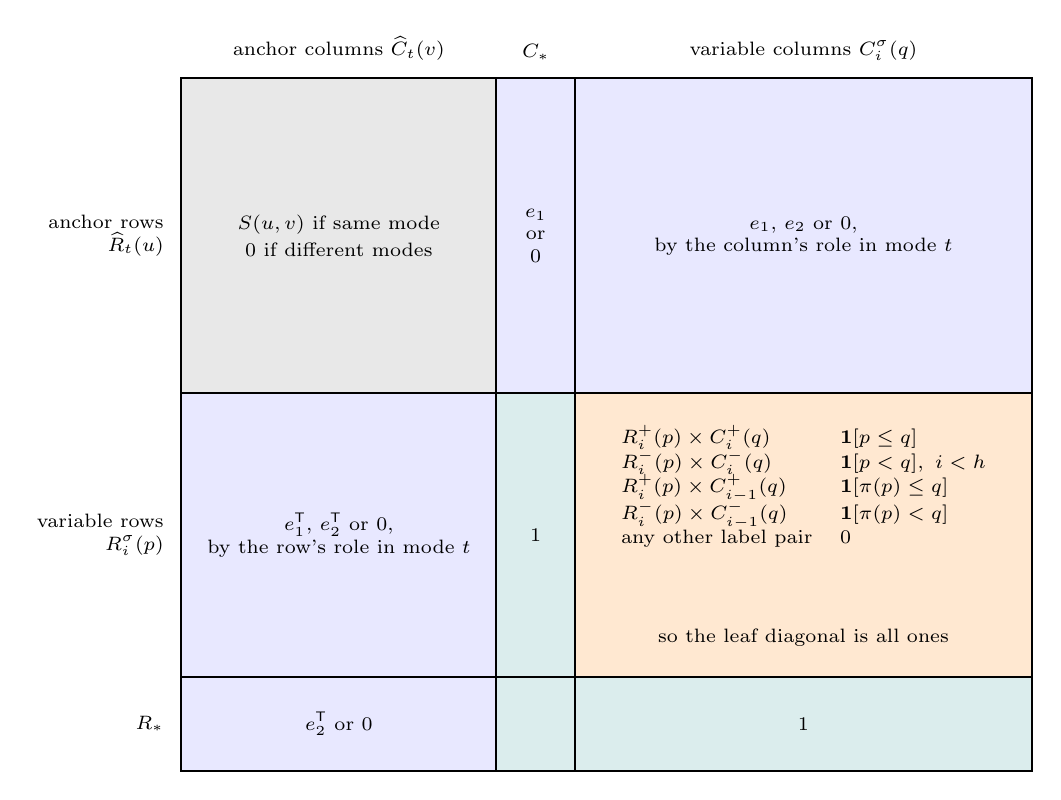
\begin{tikzpicture}[x=1cm,y=1cm,font=\scriptsize]
\fill[gray!18]   (0,0)   rectangle (4.0,-4.0);
\fill[blue!9]    (4.0,0) rectangle (10.8,-4.0);
\fill[blue!9]    (0,-4.0) rectangle (4.0,-7.6);
\fill[teal!14]   (4.0,-4.0) rectangle (5.0,-7.6);
\fill[orange!18] (5.0,-4.0) rectangle (10.8,-7.6);
\fill[blue!9]    (0,-7.6) rectangle (4.0,-8.8);
\fill[teal!14]   (4.0,-7.6) rectangle (10.8,-8.8);
\draw[thick] (0,0) rectangle (10.8,-8.8);
\draw[thick] (4.0,0) -- (4.0,-8.8);
\draw[thick] (5.0,0) -- (5.0,-8.8);
\draw[thick] (0,-4.0) -- (10.8,-4.0);
\draw[thick] (0,-7.6) -- (10.8,-7.6);
\node[above,align=center] at (2.0,0.1)  {anchor columns $\widehat C_t(v)$};
\node[above,align=center] at (4.5,0.1)  {$C_*$};
\node[above,align=center] at (7.9,0.1)  {variable columns $C_i^\sigma(q)$};
\node[left,align=right] at (-0.1,-2.0) {anchor rows\\ $\widehat R_t(u)$};
\node[left,align=right] at (-0.1,-5.8) {variable rows\\ $R_i^\sigma(p)$};
\node[left,align=right] at (-0.1,-8.2) {$R_*$};
\node[align=center] at (2.0,-2.0) {$S(u,v)$ if same mode\\[2pt] $0$ if different modes};
\node[align=center] at (4.5,-2.0) {$e_1$\\ or\\ $0$};
\node[align=center] at (7.9,-2.0) {$e_1$, $e_2$ or $0$,\\ by the column's role in mode $t$};
\node[align=center] at (2.0,-5.8) {$e_1^{\mathsf T}$, $e_2^{\mathsf T}$ or $0$,\\ by the row's role in mode $t$};
\node[align=center] at (4.5,-5.8) {$1$};
\node[align=center] at (7.9,-5.2) {%
  $\begin{array}{@{}ll@{}}
    R_i^+(p)\times C_i^+(q) & \mathbf 1[p\le q]\\
    R_i^-(p)\times C_i^-(q) & \mathbf 1[p<q],\ i<h\\
    R_i^+(p)\times C_{i-1}^+(q) & \mathbf 1[\pi(p)\le q]\\
    R_i^-(p)\times C_{i-1}^-(q) & \mathbf 1[\pi(p)<q]\\
    \text{any other label pair} & 0
  \end{array}$};
\node[align=center] at (7.9,-7.1) {so the leaf diagonal is all ones};
\node[align=center] at (2.0,-8.2) {$e_2^{\mathsf T}$ or $0$};
\node[align=center] at (7.9,-8.2) {$1$};
\end{tikzpicture}

\vspace{0.8em}

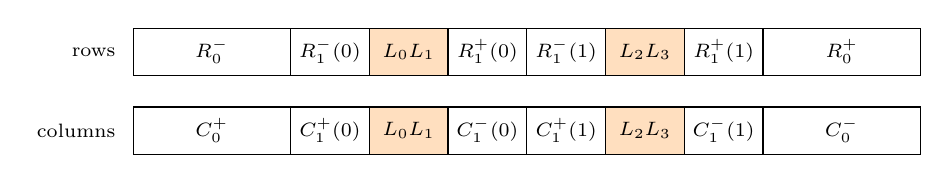
\begin{tikzpicture}[x=0.5cm,y=1cm,font=\scriptsize]
\foreach \x/\w/\lab/\c in {0/4/{$R_0^-$}/white, 4/2/{$R_1^-(0)$}/white,
  6/2/{$L_0L_1$}/orange!25, 8/2/{$R_1^+(0)$}/white, 10/2/{$R_1^-(1)$}/white,
  12/2/{$L_2L_3$}/orange!25, 14/2/{$R_1^+(1)$}/white, 16/4/{$R_0^+$}/white}
  {\fill[\c] (\x,0) rectangle (\x+\w,0.6);
   \draw (\x,0) rectangle (\x+\w,0.6);
   \node at (\x+\w/2,0.3) {\lab};}
\node[left] at (-0.2,0.3) {rows};
\foreach \x/\w/\lab/\c in {0/4/{$C_0^+$}/white, 4/2/{$C_1^+(0)$}/white,
  6/2/{$L_0L_1$}/orange!25, 8/2/{$C_1^-(0)$}/white, 10/2/{$C_1^+(1)$}/white,
  12/2/{$L_2L_3$}/orange!25, 14/2/{$C_1^-(1)$}/white, 16/4/{$C_0^-$}/white}
  {\fill[\c] (\x,-1) rectangle (\x+\w,-0.4);
   \draw (\x,-1) rectangle (\x+\w,-0.4);
   \node at (\x+\w/2,-0.7) {\lab};}
\node[left] at (-0.2,-0.7) {columns};
\end{tikzpicture}

\caption{\label{fig:map}%
}
\end{figure}

Labels are laid out on each axis in the order shown in the lower panel of
Figure~\ref{fig:map}: anchors first on both axes, then $C_*$ on the column
axis and $R_*$ last on the row axis, with the variable labels in between by
the recursion
\[
\begin{array}{llll}
\text{rows at node }(i,p): & R_i^-(p), & \text{subtree }2p,\ \text{subtree }2p{+}1, & R_i^+(p)\\[2pt]
\text{cols at node }(i,p): & C_i^+(p), & \text{subtree }2p,\ \text{subtree }2p{+}1, & C_i^-(p)
\end{array}
\]
--- the same recursion on both axes with the signs swapped. Its one
consequence, for $p,q$ at depth $i$ and $a,b$ at depth $i-1$, is
\begin{equation}\label{eq:orders}
\begin{aligned}
  R_i^+(p)<R_{i-1}^+(a)&\iff\pi(p)\le a, &
  R_{i-1}^-(a)<R_i^-(p)&\iff\pi(p)\ge a,\\
  C_{i-1}^+(b)<C_i^+(q)&\iff\pi(q)\ge b, &
  C_i^-(q)<C_{i-1}^-(b)&\iff\pi(q)\le b,
\end{aligned}
\end{equation}
so order conditions, like entries, are comparisons of node indices.

\subsection{How the two fit together}

Each of the $6h$ modes designates two row sets and two column sets:
\begin{equation}\label{eq:modes}
\begin{array}{ccccc}
 t & \mathsf R_1(t) & \mathsf R_2(t) & \mathsf C_1(t) & \mathsf C_2(t)\\[2pt]
 V_i^+ & R_i^+ & R_{i-1}^+ & C_* & C_{i-1}^+\\
 V_i^- & R_{i-1}^- & R_i^- & C_* & C_{i-1}^-\\
 W_{i,d}^+ & R_{i,d}^+ & R_* & C_{i-1}^+ & C_{i,d}^+\\
 W_{i,d}^- & R_{i,d}^- & R_* & C_{i,d}^- & C_{i-1}^-
\end{array}
\qquad 1\le i\le h,\ d\in\{0,1\},
\end{equation}
where $R_i^\sigma$ is all rows labelled $(\sigma,i,\cdot)$ and the subscript
$d$ restricts to $p\equiv d\pmod2$. These are the sets referred to by the
blue regions of Figure~\ref{fig:map}. A copy of $H$ in $A_h$ is then
\begin{enumerate}\itemsep1pt
\item one row and one column from each of the $64$ anchor groups of a single
mode $t$, realising the block $S$ of \eqref{eq:H};
\item rows $r_1<r_2$ with $r_j\in\mathsf R_j(t)$ and columns $c_1<c_2$ with
$c_j\in\mathsf C_j(t)$, these being exactly the lines whose signatures are
$e_j$;
\item such that $A_h$ restricted to $\{r_1,r_2\}\times\{c_1,c_2\}$ equals
$P$.
\end{enumerate}
Items 1--2 are addressing; item 3 is the content, and by \eqref{eq:orders}
it is a question about the threshold table phrased in node indices. Each
mode asks one such question, and $A_h$ is built so that the answer is
negative in every case but one, at the leaf diagonal. 

\subsection*{Proof}




\newpage
\section*{Extending to an infinite family of counterexamples}
\textbf{What follows is Claude's proof for infinite family of counterexamples, which I have not read through in detail yet, but Claude is confident it is correct.\\
Henning: I had my Claude review it and it believes it. I've slightly updated it} \\

We show that a counterexample $H$ with no all-zero row and no all-zero column can be enlarged
into many new counterexamples by attaching a second pattern $Z$ diagonally.

\medskip
\noindent\textbf{Setup.} Let $H$ be a $k \times l$ binary matrix and let $Z$ be a $p \times q$
binary matrix with $p, q \ge 1$. Define
\[
H' = \begin{pmatrix} H & 0 \\ 0 & Z \end{pmatrix}
\qquad \bigl((k+p) \times (l+q)\bigr),
\]
where each $0$ is a block of zeros. For an $n \times n$ binary matrix $A$, let $\widehat{Z}$ be
the matrix obtained from $Z$ by replacing every entry with a constant block of that entry having
$qn$ rows and $pn$ columns, and define
\[
A^+ = \begin{pmatrix} A & 0 \\ 0 & \widehat{Z} \end{pmatrix}.
\]
Then $\widehat{Z}$ is $pqn \times pqn$, so $A^+$ is a square matrix of size $m = (1+pq)n$. We
call its first $n$ rows and columns \emph{old} and the others \emph{new}. The new rows come in
$p$ groups of $qn$ identical rows (one group per row of $Z$), and the new columns come in $q$
groups of $pn$ identical columns (one group per column of $Z$). Every old row comes before every
new row, and every old column before every new column.

\begin{theorem}[Direct sums]\label{thm:direct}
Suppose $H$ has no all-zero row and no all-zero column, and suppose the rows of $Z$ are pairwise
distinct or the columns of $Z$ are pairwise distinct. Then for every $n \times n$ binary matrix
$A$,
\[
D_{H'}(A^+) = D_H(A)
\qquad\text{and}\qquad
N_{H'}(A^+) \le m^{p+q}\, N_H(A).
\]
\end{theorem}

\begin{corollary}\label{cor:direct}
If such an $H$ is a counterexample, then so is
$H' = \begin{pmatrix} H & 0 \\ 0 & Z \end{pmatrix}$ for every such $Z$.
\end{corollary}

The condition on $Z$ holds automatically when $Z$ has a single row or a single column. Taking
$Z = (1)$ adds one new row and one new column with a $1$ in the corner.

\section{Proof of the theorem}

Call the first $k$ rows and the first $l$ columns of $H'$ its \emph{$H$-rows} and
\emph{$H$-columns}, and the others its \emph{$Z$-rows} and \emph{$Z$-columns}.

\subsection*{Step 1: in every copy of $H'$, the $H$-part lies in the old part}

Let $X$ be any $n \times n$ binary matrix and
$M = \begin{pmatrix} X & 0 \\ 0 & \widehat{Z} \end{pmatrix}$. Take a copy of $H'$ in $M$ on rows
$r_1 < \dots < r_{k+p}$ and columns $c_1 < \dots < c_{l+q}$. We claim that
$r_1, \dots, r_k$ and $c_1, \dots, c_l$ are old, so that they form a copy of $H$ in $X$.

Suppose $r_k$ is new. Then $r_{k+1}, \dots, r_{k+p}$ are new as well. Row $k$ of $H$ contains a
$1$, say in column $j \le l$, so $M(r_k, c_j) = 1$. A new row of $M$ has $1$s only in new
columns, so $c_j$ is new, and therefore $c_{l+1}, \dots, c_{l+q}$ are new. Now look at the $p+1$
rows $r_k, r_{k+1}, \dots, r_{k+p}$ and the $q+1$ columns $c_j, c_{l+1}, \dots, c_{l+q}$. They
all lie in $\widehat{Z}$, and reading off $H'$ they carry the pattern
\[
\begin{pmatrix} 1 & 0 \\ 0 & Z \end{pmatrix}.
\]
If the rows of $Z$ are pairwise distinct, the $p+1$ rows of this pattern are pairwise distinct:
the first row differs from the others in its first entry. But the new rows form only $p$
groups, so two of our $p+1$ rows lie in the same group, and two rows of $M$ in the same group
are identical. This is a contradiction. If instead the columns of $Z$ are pairwise distinct, the
same argument works with the $q+1$ columns and the $q$ groups of new columns. Hence $r_k$ is
old, and so are $r_1, \dots, r_k$.

Finally suppose $c_l$ is new. Column $l$ of $H$ contains a $1$, say in row $i \le k$, so
$M(r_i, c_l) = 1$. But $r_i$ is old, and an old row has $1$s only in old columns, a
contradiction. Hence $c_1, \dots, c_l$ are old.

\subsection*{Step 2: the count, and $D_{H'}(A^+) \le D_H(A)$}

By Step 1 with $X = A$, every copy of $H'$ in $A^+$ consists of a copy of $H$ in $A$ together
with $p$ more rows and $q$ more columns, for which there are at most $m^{p+q}$ choices. Hence
$N_{H'}(A^+) \le m^{p+q} N_H(A)$.

Next, change $D_H(A)$ entries of $A$ to get an $H$-free matrix $A_0$, and leave the rest of
$A^+$ unchanged. By Step 1 with $X = A_0$, the result has no copy of $H'$. Hence
$D_{H'}(A^+) \le D_H(A)$.

\subsection*{Step 3: $D_{H'}(A^+) \ge D_H(A)$}

Let $B$ be any $m \times m$ binary matrix with no copy of $H'$. Let $E_0$, $E_1$, $E_2$ be the
numbers of entries where $B$ differs from $A^+$ in the old-old block, in the two mixed blocks,
and in the new-new block. We must show $E_0 + E_1 + E_2 \ge D$, where $D = D_H(A)$. Note
$D \le n^2$, since the zero matrix has no copy of $H$ ($H$ contains a $1$).

Pick one row uniformly at random from each of the $p$ groups of new rows, and one column
uniformly at random from each of the $q$ groups of new columns, all independently. Call these
the \emph{picked} rows $\rho_1 < \dots < \rho_p$ and columns $\gamma_1 < \dots < \gamma_q$. Call
the pick \emph{good} if $B$ agrees with $A^+$ on all $pq$ entries $(\rho_i, \gamma_j)$, that is,
if $B(\rho_i, \gamma_j) = Z(i,j)$ for all $i, j$. A fixed new-new entry is picked with
probability $\frac{1}{qn \cdot pn}$, so by the union bound
\[
\Pr[\text{the pick is not good}] \le \frac{E_2}{pq\,n^2}.
\]

Call an old row $r$ \emph{bad} if $B(r, \gamma_j) = 1$ for some $j$, and an old column $c$
\emph{bad} if $B(\rho_i, c) = 1$ for some $i$. Each such $1$ is one of the $E_1$ changed entries
in the mixed blocks, since those blocks are $0$ in $A^+$. Each changed entry lies on a picked
line with probability $\frac{1}{pn}$ or $\frac{1}{qn}$, hence at most $\frac{1}{n}$. So the
expected number of bad rows and columns is at most $E_1/n$.

Let $B^\circ$ be the old-old block of $B$ with every bad row and bad column replaced by zeros.
This changes at most $n$ entries per bad line, so $B^\circ$ differs from $A$ in at most
$E_0 + W$ entries, where $W$ is $n$ times the number of bad lines and has expectation at most
$E_1$.

\emph{Claim: if the pick is good, $B^\circ$ is $H$-free.} Suppose it has a copy of $H$ on rows
$r_1 < \dots < r_k$ and columns $c_1 < \dots < c_l$. Every row and column of $H$ contains a $1$,
so none of these rows or columns was replaced by zeros. Thus none of them is bad, and on these
entries $B^\circ$ agrees with $B$. Not being bad means $B(r_a, \gamma_j) = 0$ and
$B(\rho_i, c_b) = 0$ for all indices, and the pick being good means
$B(\rho_i, \gamma_j) = Z(i,j)$. Since old rows and columns come before new ones, the rows
$r_1, \dots, r_k, \rho_1, \dots, \rho_p$ and the columns
$c_1, \dots, c_l, \gamma_1, \dots, \gamma_q$ form a copy of $H'$ in $B$, which is impossible.
This is the only place where the assumption on $H$ is used beyond Step 1.

By the claim, whenever the pick is good we have $D \le E_0 + W$. Taking expectations,
\[
D \left(1 - \frac{E_2}{pq\,n^2}\right) \le D \cdot \Pr[\text{good}] \le E_0 + \mathbb{E}[W]
\le E_0 + E_1 .
\]
Rearranging and using $D \le n^2 \le pq\,n^2$,
\[
E_0 + E_1 + E_2 \;\ge\; D + E_2\left(1 - \frac{D}{pq\,n^2}\right) \;\ge\; D .
\]
Since $B$ was arbitrary, $D_{H'}(A^+) \ge D_H(A)$. Together with Step 2 this proves the
theorem. \qed

\begin{remark}
The probability argument is an average over the $(qn)^p (pn)^q$ possible picks, all equally
likely. In a formal proof it can be replaced by double counting: sum the inequality
``$\mathbf{1}[\text{good}]\cdot D \le E_0 + W$'' over all picks.
\end{remark}

\section{Proof of the corollary}

Fix $c', C' > 0$; we must find a host showing that $c'$ and $C'$ do not work for $H'$. Put
$s = 1 + pq$, $C = C'$ and $c = c'\, s^{k+l-2C'}$. Since $H$ is a counterexample, there are $n$, an $n \times n$ matrix $A$
and $\epsilon \in (0,1]$ with $\dist_H(A) \ge \epsilon$ and $N_H(A) < c\,\epsilon^C n^{k+l}$.
Let $m = sn$ and $\epsilon' = \epsilon/s^2 \in (0,1]$. By the theorem,
\[
\dist_{H'}(A^+) = \frac{D_H(A)}{(sn)^2} \ge \frac{\epsilon}{s^2} = \epsilon'
\]
and, using $n = m/s$ and $\epsilon = s^2 \epsilon'$,
\[
N_{H'}(A^+) \le m^{p+q} N_H(A) < c\,\epsilon^{C} n^{k+l} m^{p+q}
= c\, s^{2C}(\epsilon')^{C}\, s^{-(k+l)}\, m^{(k+p)+(l+q)}
= c'\,(\epsilon')^{C'}\, m^{(k+p)+(l+q)} .
\]
So $c'$ and $C'$ fail for $H'$ on the host $A^+$. As $c'$ and $C'$ were arbitrary, $H'$ is a
counterexample. \qed

\medskip
If ``counterexample'' is read in the stronger form, with hosts of arbitrarily large size $n$
for a fixed $\epsilon$, the same proof applies: $m = sn$ grows with $n$, and $\epsilon/s^2$ is
fixed.

\section{Variant: appending zero rows or zero columns}

Let $H'$ be $H$ with $q \ge 1$ all-zero columns appended on the right, and let
$A^+ = \begin{pmatrix} A & 0 \\ 0 & 0 \end{pmatrix}$ have size $m = (1+q)n$. Then again
$D_{H'}(A^+) = D_H(A)$ and $N_{H'}(A^+) \le m^{q} N_H(A)$, so the corollary holds for this
$H'$ as well. The proof is a simpler version of the one above.
\begin{itemize}
\item \emph{Step 1.} Every row and every $H$-column of $H'$ contains a $1$, and the only $1$s
of $M = \begin{pmatrix} X & 0 \\ 0 & 0 \end{pmatrix}$ are in the old-old block, so the $H$-part
of any copy is old.
\item \emph{Step 3.} Split the $qn$ new columns into $q$ groups of $n$, pick one column from
each group, call an old row bad if $B$ has a $1$ where it meets a picked column, and replace
bad rows by zeros. No event ``good'' is needed, and one gets $D \le E_0 + E_1$ directly.
\end{itemize}
The same holds for appending $p$ all-zero rows at the bottom, by exchanging rows and columns.

\section{Remarks}

\begin{itemize}
\item \emph{Symmetries.} Swapping $0$s and $1$s, reversing the order of the rows, reversing the
order of the columns, and transposing all preserve $N_H$ and $D_H$ when applied to both $H$ and
$A$. So the theorem has a dual form (if $H$ has no all-ones row or column, fill the
off-diagonal blocks with $1$s), and $Z$ can be attached at any of the four corners.

\item \emph{New counterexamples.} OpenAI's $66 \times 66$ matrix $H$ has no all-zero row and no
all-zero column (every row and column of its anchor contains a $1$, and so do its marks and its
body). Hence $\begin{pmatrix} H & 0 \\ 0 & Z \end{pmatrix}$ is a counterexample for every $Z$
with pairwise distinct rows or pairwise distinct columns, for example $Z = (1)$, $Z = (0)$ or
$Z = (1\ 0)$, and $H$ with one appended zero column is a $66 \times 67$ counterexample. The same
applies to the smaller counterexamples found since, all of which have no all-zero row or column;
among them Shea's claimed $3 \times 3$ counterexample
$K = \begin{pmatrix} 0&1&1\\1&0&1\\1&1&0 \end{pmatrix}$ (an unrefereed manuscript), which
would give, for instance,
\[
\begin{pmatrix} 0&1&1&0\\1&0&1&0\\1&1&0&0\\0&0&0&1 \end{pmatrix}
\qquad\text{and}\qquad
\begin{pmatrix} 0&1&1&0\\1&0&1&0\\1&1&0&0 \end{pmatrix}.
\]

\item \emph{Sub-patterns do not help.} Every $Z$ with pairwise distinct rows, including patterns
for which polynomial removal is known to hold such as the $2 \times 2$ identity, appears as a
diagonal block of a counterexample.

\item \emph{Credit.} For identity matrices this is Lupini's padding lemma (Zenodo record
23618367, Lemma ``Identity padding''): $I_k = \operatorname{diag}(I_\ell, I_p)$, with each new
diagonal $1$ blown up to an $n \times n$ block of ones, so $H = I_\ell$ and $Z = I_p$. Step 3
follows his argument. The observation here is that his proof needs only that $H$ has no
all-zero row or column, and that the attached block can be an arbitrary $Z$ with pairwise
distinct rows or columns.

\item \emph{Checks.} Both statements of the theorem and of the variant were verified by exact
computation on small hosts: $120$ direct sums with $2 \times 2$ patterns $H$ and
$Z \in \{(1), (0), (1\ 0), (0\ 1)^{T}, (1\ 1)\}$ ($41$ of them with $D_H(A) > 0$), and $80$
zero-column variants, with no failure (\texttt{scratch/direct-sum/check.py}). These checks are a
sanity test, not part of the proof. A Lean proof of the theorem and the corollary, with
$H$ rectangular as here, is in \texttt{lean/OrderedRemoval/Statements.lean}. The folder
\texttt{lean-unconditional/} combines it with OpenAI's Lean proof for their $66 \times 66$
example (Apache-2.0, credited there).
\end{itemize}

\section*{An infinite family of examples}
\subsection*{Repeated rows and columns do not matter}

Let $H$ be a $k\times l$ pattern. Delete any row that equals the row just above it, and any column that
equals the column just to its left, and repeat until nothing can be deleted. Call the result
$R=\operatorname{red}(H)$, of size $k_0\times l_0$. For example,
\[
 \operatorname{red}\begin{pmatrix}1&1&0\\1&1&0\\0&0&1\end{pmatrix}=\begin{pmatrix}1&0\\0&1\end{pmatrix}.
\]
(For a pattern that is not square, read the conjecture with $n^{k+l}$ in place of $n^{2k}$.)

\textbf{Theorem.} $H$ satisfies the conjecture if and only if $\operatorname{red}(H)$ does.

\medskip
The proof rests on two facts.

\textbf{Fact 1 (many copies of $H$ give many copies with one more repeat).}
Let $H'$ be $H$ with column $j$ written twice in a row. Then for every $n\times n$ matrix $B$,
\[
 N_{H'}(B)\ \ge\ \frac{N_H(B)^2}{2n^{k+l-1}}-\frac{N_H(B)}{2}.
\]
The same holds for a repeated row.

\emph{Proof.} Take an $n \times n$ matrix. Fix some $k$ rows and the $l-1$ columns of a copy of $H$; call this a \emph{frame}. Let $x$
be the number of columns that complete the frame to a copy of $H$. The frame gives $x$ copies of $H$ and
$\binom{x}{2}$ copies of $H'$, since the two equal columns of $H'$ can be any two of these $x$ columns. There are
at most $n^{k+l-1}$ frames, and $\binom{x}{2}$ is convex in $x$, so the bound follows from Jensen's inequality.
$\square$

\medskip
\textbf{Fact 2 (blowing up a host).}
Let $A$ be $n\times n$, and let $A^{(q)}$ be the $qn\times qn$ matrix obtained by replacing every entry of $A$
with a constant $q\times q$ block. Then
\begin{align*}
 \text{(a)}\quad & \frac{N_H(A^{(q)})}{(qn)^{k+l}}\ \le\ \frac{N_R(A)}{n^{k_0+l_0}},\\[2pt]
 \text{(b)}\quad & D_H(A^{(q)})\ \ge\ \tfrac12\,q^2\,D_R(A)\quad\text{for all large enough } q.
\end{align*}

\emph{Proof of (a).} Inside a copy of $H$ in $A^{(q)}$, keep one row and one column for each row and column of
$R$. This is a copy of $R$. Two of its rows cannot come from the same block of $q$ equal rows: then two
neighbouring rows of $R$ would be equal. The same holds for columns. So the copy of $R$ comes from a copy of $R$
in $A$, and each copy of $R$ in $A$ is counted at most $q^{k_0+l_0}(qn)^{k+l-k_0-l_0}$ times.

\emph{Proof of (b).} Change at most $\frac12q^2D_R(A)$ entries of $A^{(q)}$ and call the result $B'$. We show
that $B'$ still contains $H$. Pick one row from each block of rows and one column from each block of columns
at random. The picked rows and columns form an $n\times n$ matrix $B$. Each changed entry is picked with
probability $1/q^2$, so on average $B$ differs from $A$ in at most $D_R(A)/2$ entries. Hence with probability
at least $\frac12$ it differs in fewer than $D_R(A)$ entries, and then $B$ contains a copy of $R$. A given
copy of $R$ in $B'$ is picked with probability $q^{-(k_0+l_0)}$, so
\[
 N_R(B')\ \ge\ \tfrac12\,q^{k_0+l_0}.
\]
So a fixed positive fraction (depending on $n$, not on $q$) of all possible positions holds a copy of $R$ in
$B'$. Applying Fact~1 once for each repeated row or column, the same is true for $H$ when $q$ is large. In
particular $B'$ contains $H$. $\square$

\medskip
\emph{Proof of the Theorem.}

\emph{If $R$ satisfies the conjecture, so does $H$.} Let $\operatorname{dist}_H(A)\ge\epsilon$. Since $H$
contains $R$, every $R$-free matrix is $H$-free, so $\operatorname{dist}_R(A)\ge\epsilon$ and $A$ has at least
$c\,\epsilon^Cn^{k_0+l_0}$ copies of $R$. Applying Fact~1 once for each repeated row or column gives at least
$c'\epsilon^{C'}n^{k+l}$ copies of $H$. (This needs $n$ larger than a fixed power of $1/\epsilon$; for smaller
$n$ use $N_H(A)\ge1$ and a larger $C'$.)

\emph{If $R$ fails the conjecture, so does $H$.} Let $c',C'>0$ be given. Since $R$ fails, there is a matrix
$A$ with $\operatorname{dist}_R(A)\ge\epsilon_0$ and fewer than $c'2^{-C'}\epsilon_0^{C'}n^{k_0+l_0}$ copies of
$R$. By Fact~2, for large $q$ the matrix $A^{(q)}$ satisfies
$\operatorname{dist}_H(A^{(q)})\ge\epsilon_0/2=:\epsilon$ and has fewer than $c'\epsilon^{C'}(qn)^{k+l}$ copies
of $H$. So no constants $c',C'$ work for $H$. $\square$

\medskip
\textbf{Examples.}
\begin{itemize}
\item Any pattern made of two all-ones blocks in opposite corners and zeros elsewhere reduces to the
 $2\times2$ identity (or its mirror image), so it satisfies the conjecture by Lupini's theorem.
\item Shea's crown with any rows or columns repeated still fails the conjecture.
\end{itemize}

 \begin{thebibliography}{99}
 
  \bibitem{ABE}   
  N.~Alon and O.~Ben-Eliezer, \emph{Efficient removal lemmas for matrices},
  Order \textbf{37} (2020), no.~1, 83--101, doi:10.1007/s11083-019-09494-3, arXiv:1609.04235.
  
  \bibitem{ABF17}
  N.~Alon, O.~Ben-Eliezer, and E.~Fischer, \emph{Testing hereditary properties of ordered graphs and matrices}, 2017 IEEE 58th Annual Symposium on Foundations of Computer Science (FOCS), 2017, pp.~848--858, doi:10.1109/FOCS.2017.83, arXiv:1704.02367.                                                                                             
  \bibitem{AFN}            
  N.~Alon, E.~Fischer, and I.~Newman, \emph{Efficient testing of bipartite
  graphs for forbidden induced subgraphs}, SIAM J. Comput. \textbf{37} (2007),
  no.~3, 959--976, doi:10.1137/050627915.

  \bibitem{erebos}
  Erebos Labs, \emph{ordered-matrix-removal-4x4}, Lean formalization of a
  $4\times4$ obstruction, GitHub release v1.0.0, 9 October 2026,
  \url{https://github.com/erebos-labs/ordered-matrix-removal-4x4}.

  \bibitem{GS}
  L.~Gishboliner and A.~Shapira, \emph{Polynomial property testing},
  Comput. Sci. Rev. \textbf{58} (2025), 100806,
  doi:10.1016/j.cosrev.2025.100806, arXiv:2508.16878.

  \bibitem{Lupini}
  Lupini, Martino. \emph{Polynomial Removal for the Ordered Two-by-Two Identity Matrix}, preprint, Zenodo, November 2, 2026,
  \url{https://doi.org/10.5281/zenodo.23618366}.


  \bibitem{openai}
  OpenAI, \emph{Polynomial removal fails for ordered binary matrices},
  preprint, 25 September 2026,
  \url{https://github.com/openai/math/tree/main/preprints/Polynomial-removal-fails-for-ordered-binary-matrices-September-25-2026}.

  \bibitem{proveit}
  ProveIt project, \emph{A $5\times5$ obstruction to polynomial ordered matrix
  removal}, draft, 7 October 2026,
  \url{https://github.com/VladimirReshetnikov/ProveIt/tree/bfbfe915186310fdf745a7a089e7dd88eeb773b1/Combinatorics/OrderedMatrices/Research/ordered-matrix-removal}.

  \bibitem{shea}
  R.~Shea, \emph{A $3\times3$ ordered binary matrix removal obstruction},
  manuscript, 12 October 2026,
  \url{https://github.com/shea256/ordered-binary-matrix-removal}.

  \bibitem{wang}
  Z.~Wang, \emph{A four-by-four obstruction to polynomial removal for ordered
  binary matrices}, preprint, 11 October 2026, arXiv:2610.15370.

  \end{thebibliography}

\end{document}
